\documentclass[../main.tex]{subfiles}
\usepackage{amsmath, bm}
\usepackage{graphicx}
\begin{document}

\noindent
본 챕터에서는 지금까지의 챕터에서 설명한 각종 기법을 취합하여 대어휘 연속 음성 인식 (large vocabulary continuous speech recognition; LVCSR) 엔진을 구성하는 방법에 대해 설명한다. 

\section{FST의 합성과 확률모델}
지금까지 도입했던 음성인인식의 요소를 나타내는 FST를 합성하고, 합성한 FST의 최단 경로 문제의 풀이로서 음성인식결과를 얻는 방법을 고찰한다. 음성인식의 통계모델을 표현하는 FST는 일반적으로는 아래의 4 종류가 있다. 

\begin{itemize}
    \item \textbf{\textit{G}}: 단어열 Acceptor (\hyperref[sec:N-gram-FST]{6.5})
    \item \textbf{\textit{L}}: 문맥에 의존하지 않는 음소열로부터 단어열 변환 (\hyperref[subsec:pronunciation-model]{4.2.2})
    \item \textbf{\textit{C}}: 문맥에 의존하는 음소열로부터 문맥에 의존하지 않는 음소열로 변환 (\hyperref[sec:context-dependant-model]{5.3})
    \item \textbf{\textit{H}}: HMM state 시퀀스로부터 문맥에 의존하는 음소열로 변환 (\hyperref[sec:context-dependant-model]{5.3})
\end{itemize}
여기에 덧붙여서, 이하의 식에서 보여지고 있는 입력 (관측 벡터열)과 HMM 상태변수의 관계를 나타내는 FST \textbf{\textit{E}}를 가상으로 도입함으로써, 인식할 때의 처리를 모두 FST 형식으로 기술할 수 있게 된다. 

\begin{equation}\label{eq:7-1}
    \begin{split}
    Q[\bm{E}] &= \{0,\ldots,T\}, \qquad I[\bm{E}] = \{(0,\bar{1})\}, \qquad F[\bm{E}] = \{(T,\bar{1})\}, \\
    E[\bm{E}] &= \{(t-1, t, \sigma, \sigma, -\log p(\mathbf{x_t} | s_t = \sigma)): t \in {1, \ldots, T}, \sigma \in \Sigma[\bm{H}] \}
    \end{split}
\end{equation}

여기에서 \textit{T}는 관측 벡터열의 길이를 의미한다. 

음성인식 전체의 변환처리, 이른바 입력 프레임 시퀀스에서 단어열로의 변환은, 이 모든 FST를 합성한 $\bm{E} \circ \bm{H} \circ \bm{C} \circ \bm{L} \circ \bm{G}$로 나타낼 수 있다.
또한 그 FST의 변환 결과로써 가장 가중치가 작아지는 가설은 최단경로문제를 푸는 것으로써 근사적으로 구할 수 있다.
\hyperref[sec:HMM]{5.1}에서 설명한 바와 같이, 이를 Viterbi 디코딩이라 한다. 
그러나 많은 경우에, 이 FST는 거대하여, Viterbi 디코딩과 같은 근사적 해법으로도 풀기가 어렵다. 
대어휘 연속 음성인식기술은, 이런 거대한 FST 위에서, Viterbi 디코딩을 가능케하는 기술이라 할 수 있다. 

\subsection{디코딩 네트워크의 구성과 탐색오류}

입력에 의존하는 $\bm{E}$를 제외한 나머지 모두를 합성한 FST가 음성인식에서 사용되는데, 이 FST를 디코딩 네트워크라고 부르고, $\bm{D}$로 나타낸다. 

\begin{equation}
    \bm{D} = \bm{H} \circ \bm{C} \circ \bm{L} \circ \bm{G}
\end{equation}

위의 식에서 $\bm{H}$, $\bm{C}$, $\bm{L}$, $\bm{G}$는 각각 출력분포를 제외한 음향모델로, 음소 문맥 클러스터링, 발음모델, 언어모델에 해당한다고 할 수 있다. 
디코딩 네트워크는 입력에 대해서는 변하지 않으면서, 합성과 최적화를 다시 계산해 두는 것이 가능하다. 
음성인식은 출력분포를 나타내는 FST $\bm{E}$와 디코딩 네트워크 $\bm{D}$의 합성 FST를 계산해가면서, 그 최단 경로를 탐색하는 문제로 불 수 있다. 
따라서 등가성을 유지한 채로 $\bm{D}$에 대해 가능한한 작고 간단하게 바꿔 표현하는 것은 탐색효율 향상을 위해 중요하다. 

대어휘 연속 음성인식에서는 디코딩 네트워크가 크기 때문에 엄밀한 최단 경로 탐색을 수행하는 것은 가능하지 않다. 
뒤에서 언급할 빔 탐색 알고리즘은 최단 경로 문제의 근사적 해법이지만, 이런 알고리즘에는 근사 정확성과 계산량 사이에 트레이드오프가 존재한다. 
디코딩 네트워크를 최적화하고 최단 경로 문제의 규모를 축소함으로써, 같은 계산량이더라도 보다 높은 정확성을 갖는 근사 탐색을 수행할 수 있으며, 음성인식의 정확도 형상에도 기여한다. 

최단 경로 탐색의 근사에 기인하는 오류를 탐색 오류 (search error)라고 부른다. 
탐색 오류는 계산량의 제약을 무시하고 근사 정확도를 최대로 높이는 경우의 음성인식 결과와, 실제 응용 상의 계산 효율을 고려한 근사를 이용한 경우의 음성인식 결과를 비교하여 평가할 수 있다. 
\hyperref[fig:7_1]{그림 7.1}에서 탐색 알고리즘의 근사 정도를 나타내는 파라미터 (빔폭; 자세히는 뒤에 설명)과 단어오류율의 관계를 나타낸다. 
빔폭을 충분히 크게 설정하게 되면 탐색오류는 줄어들게 되고, 모델 자체에 의한 오류만 남게 된다. 
따라서 실제로 사용되는 빔폭을 설정했을 때의 오류율과 모델 자체의 오류율을 비교함으로써 탐색처리의 근사에 의해 생기는 오류 정도를 평가할 수 있게 된다. 

\begin{figure}[h]
    \centering
    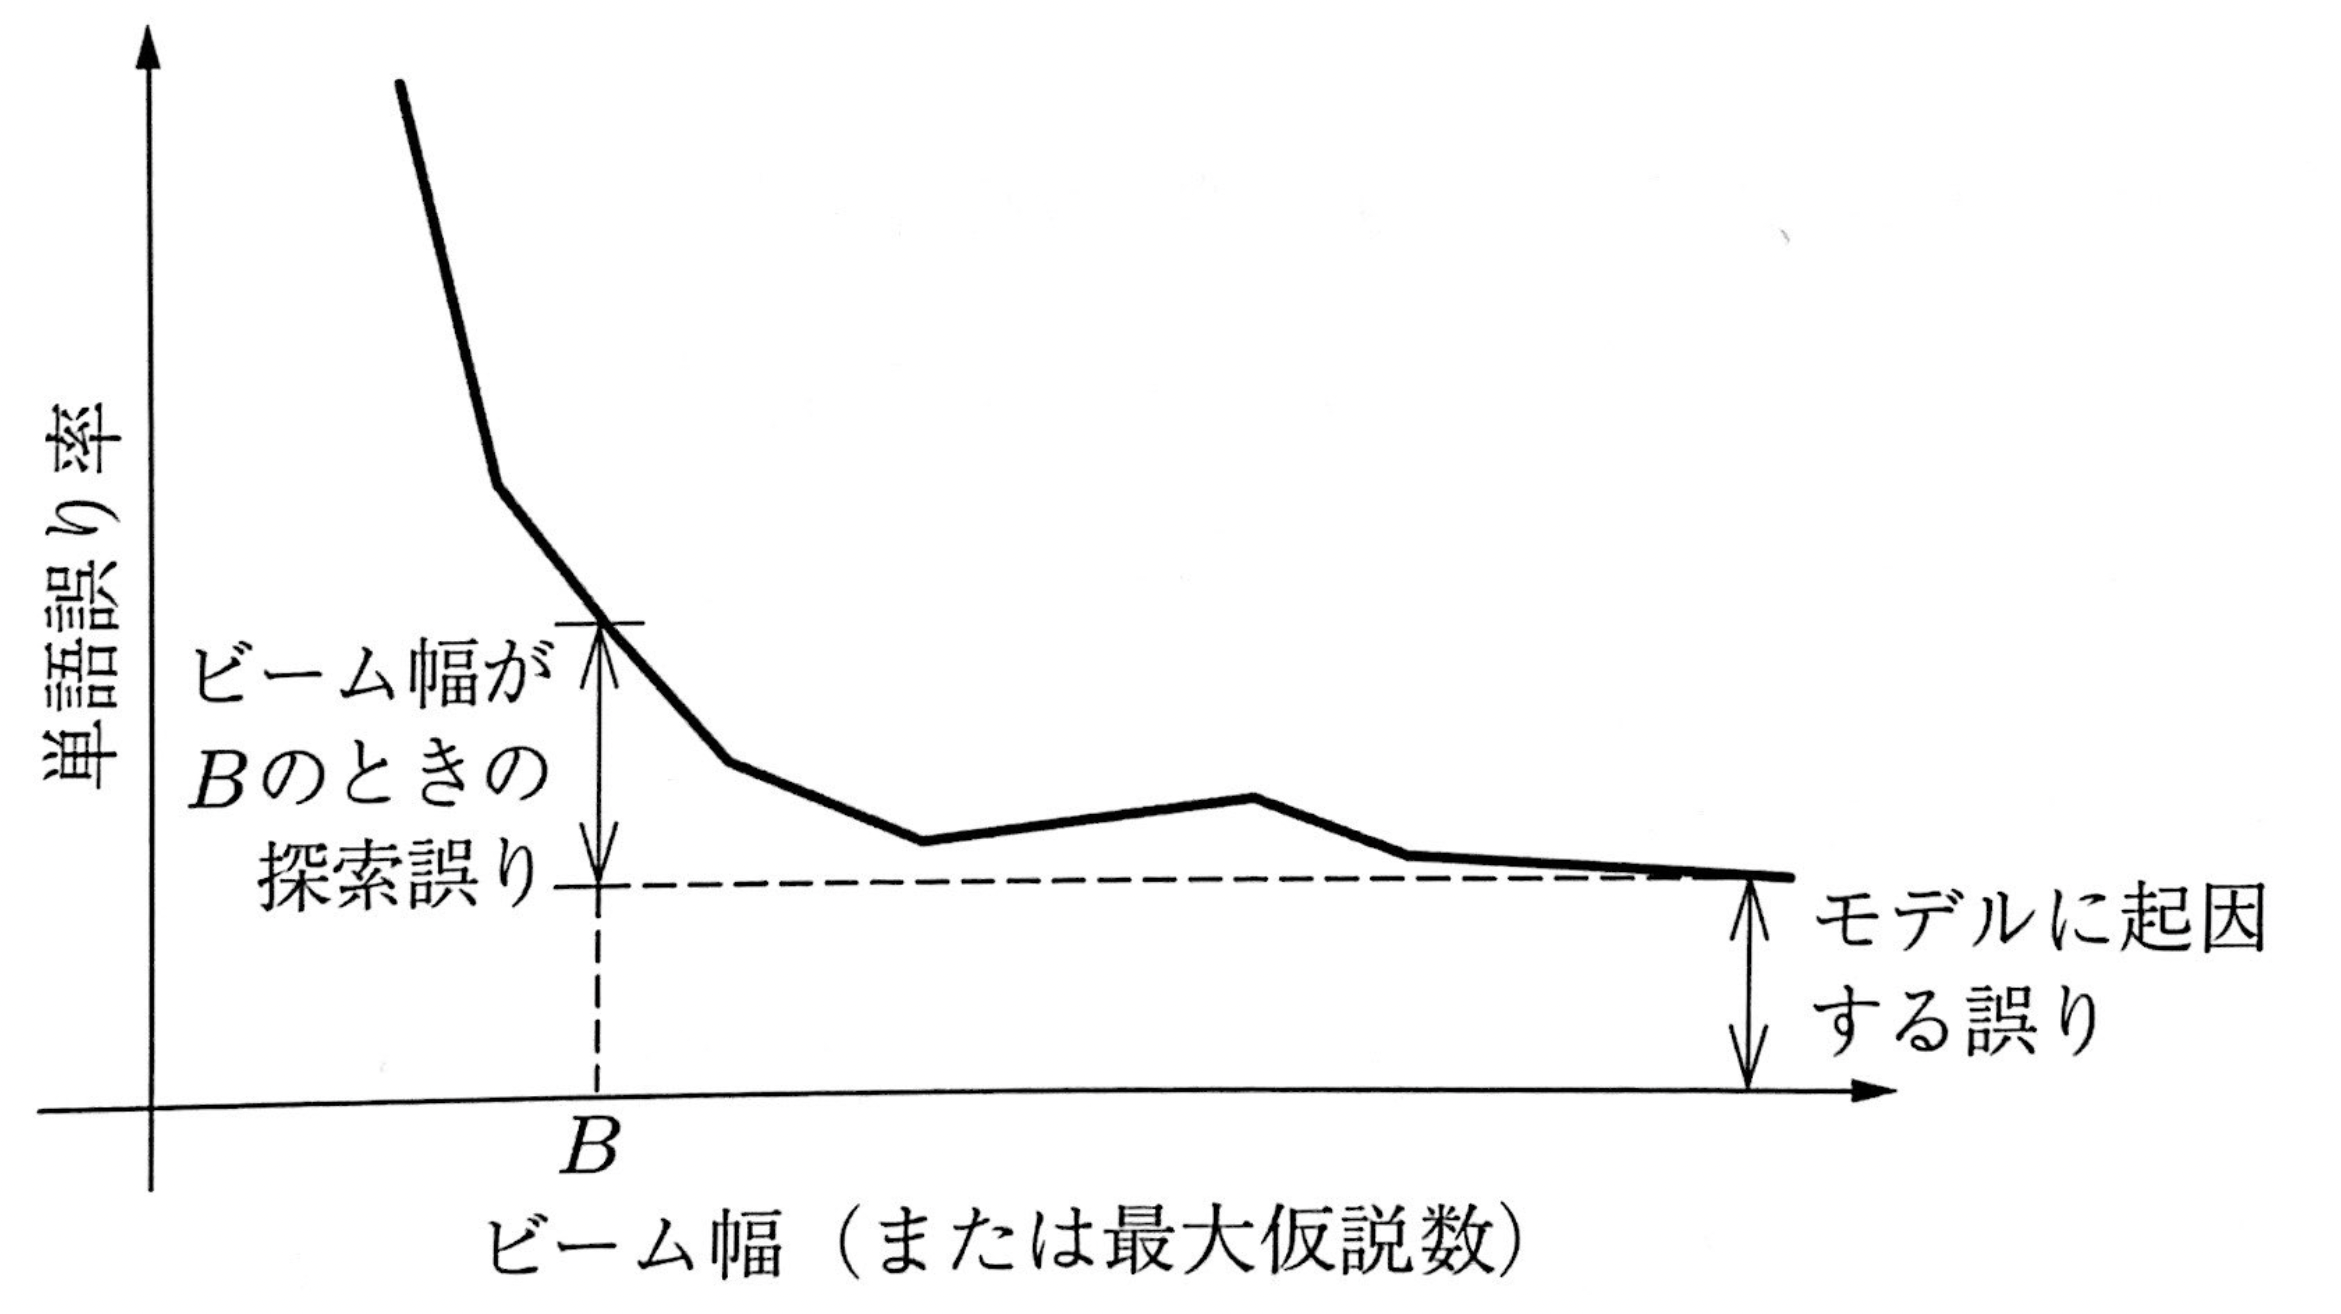
\includegraphics[width=10cm]{../figures/fig7_1_orig}\label{fig:7_1}
    \caption{탐색오류와 빔폭의 관계}
\end{figure}


디코딩 네트워크를 효율적인 표현으로 바꿈으로써, 탐색 알고리즘의 효율을 향상시켜서, 결과적으로 평가에 있어서 같은 계산 자원으로 보다 적은 탐색오류를 달성할 수 있게 된다. 

\subsection{disambiguation 심볼}
대어휘 연속 음성인식에 있어서의 FST의 최적화에서는 결정화 (와 그 전처리로써 필요한 $\epsilon$제거) 및 최소화가 이루어진다. 
FST의 최적화 (Opt라고 한다)는 예를 들어 아래와 같은 것으로, 3개의 FST 변환 함수에 의해 나타낼 수 있다. 

\begin{equation}
    \text{Opt}(\bm{X}) \stackrel{\text{def}}{=} \text{Min}(\text{Det}(\text{RmEps}(\bm{X})))
\end{equation}

여기서 RmEps는 $\epsilon$제거 (\hyperref[subsec:epsilon-remove]{3.6.2}), Det는 결정화 (\hyperref[subsec:determinization]{3.6.4}), Min은 최소화 (\hyperref[subsec:minimization]{3.6.5})를 의미한다. 

이와 같은 최적화 연산에 의해서 등가 교환이 가능한 FST 가운데 가장 작은 결정성 FST를 얻을 수는 있으나, 결정성 FST는 잘 설계된 비결정성 FST에 비해서 상태수가 많은 경우도 있고, 디코딩 네트워크 전체를 결정성 FST로 표현하는 것이 어렵다.\footnote{예를 들어 \hyperref[sec:N-gram-FST]{6.5}의 방법에 의해 백오프나 보간 구조를 사용하여 구성한 N그램 언어모델의 FST를 결정화하는 것은 상태 갯수의 조합이 폭발적으로 늘어나기 때문에 많은 경우에 어렵다.}
게다가 디코딩 네트워크를 구성하는 각 요소의 결정화와 최소화를 수행함으로써 최종적인 디코딩 네트워크를 작게 유지하는 것을 생각할 수 있다. 

결정화는 같은 접두사를 갖는 상태를 공유하는 효과가 있기 때문에, 특히 $\bm{L}$과 $\bm{C}$에 있어서는 상태의 갯수를 줄이는 효과를 기대할 수 있다. 
실용적인 상태 갯수의 결정성 FST를 얻을 수 있다면, 최소화 처리에 의해 상태 갯수를 더욱 줄이는 것이 가능하다. 
그러나 결정화가 가능하다는 것은 함수형 FST, 이른바 어떤 입력 시퀀스에 대해 단 하나의 출력 시퀀스만 가능한 FST로 한정되는데, 예를 들어 $\bm{L}$은 동음이의어를 갖는 경우, 이 전제를 만족할 수 없게 된다. 
이 때 도입할 수 있는 것이 disambiguation 심볼이다. 

\begin{figure}[h]
    \centering
    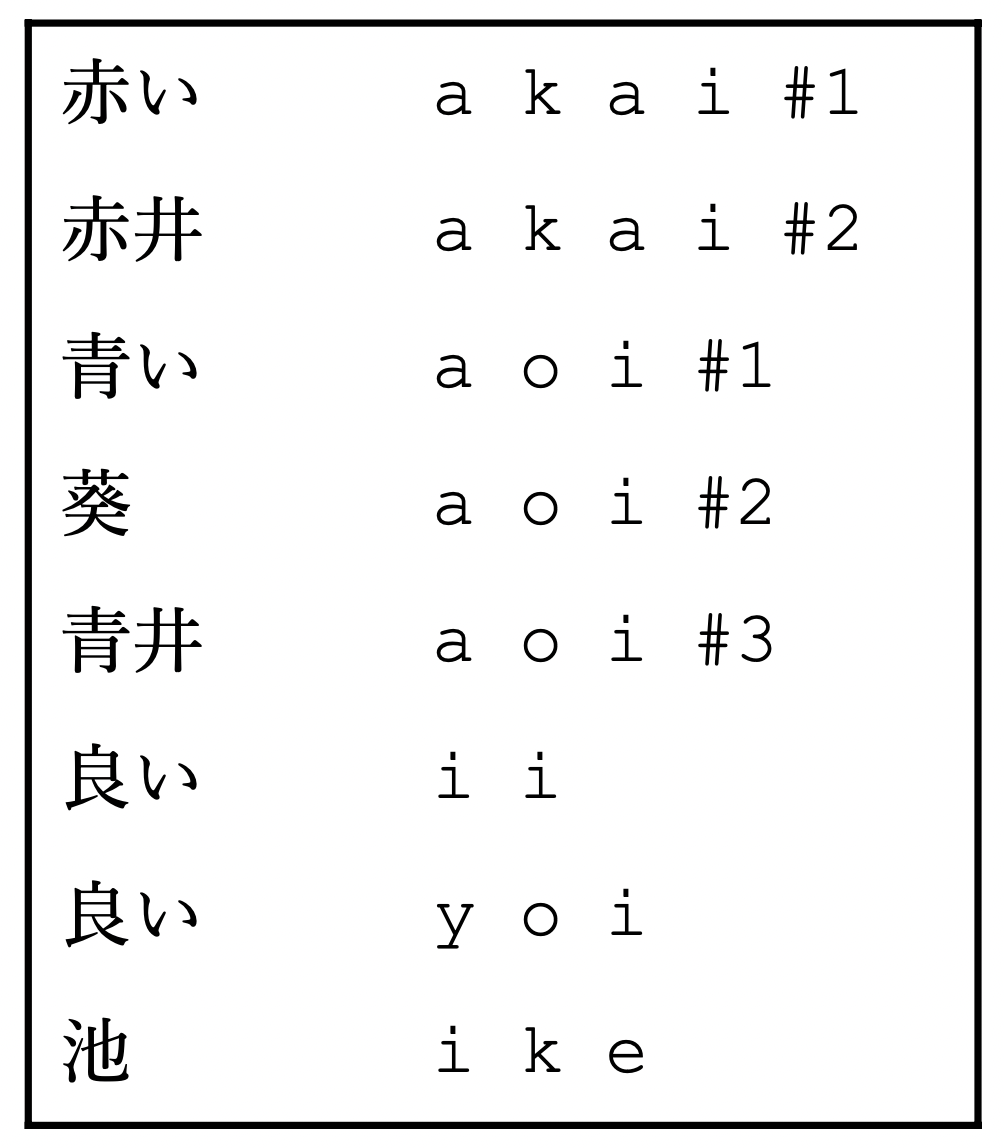
\includegraphics[width=5cm]{../figures/fig7_2_orig.png}\label{fig:7_2}
    \caption{disambiguation 심볼을 적용한 렉시콘}
\end{figure}

\hyperref[fig:7_2]{그림 7.2}에서는 disambiguation 심볼을 도입한 렉시콘의 예를 보여주고 있다. 
disambiguation 심볼은 \hyperref[fig:7_2]{그림}에서는 \texttt{\#1}과 \texttt{\#2}가 있는데, 이는 렉시콘 내의 동음이의어를 구별하기 위해 필요한 만큼 준비할 수 있다. 
\hyperref[fig:7_2]{그림}에서의 렉시콘의 경우, \texttt{/a o i/}에 대응하는 단어가 가장 많으며 그 수는 3개이기 때문에 \texttt{\#1}부터 \texttt{\#3}까지 disambiguation 심볼로써 추가할 수 있다. 
이런 심볼을 도입함으로써 렉시콘 FST를 결정화할 수 있다. 



\section{대어휘 연속 음성인식의 탐색문제}

\section{대규모 FST 합성 기술}
\subsection{온 더 플라이 합성}
\subsection{디스크 기반 인식 시스템}

\section{N-Best 리스트 및 lattice 생성}
\subsection{lattice 생성}
\subsection{lattice로부터 N-Best 리스트 생성}

\section*{인용 및 참고문헌}

\end{document}
